% Created by tikzDevice version 0.10.1 on 2016-02-27 13:23:44
% !TEX encoding = UTF-8 Unicode
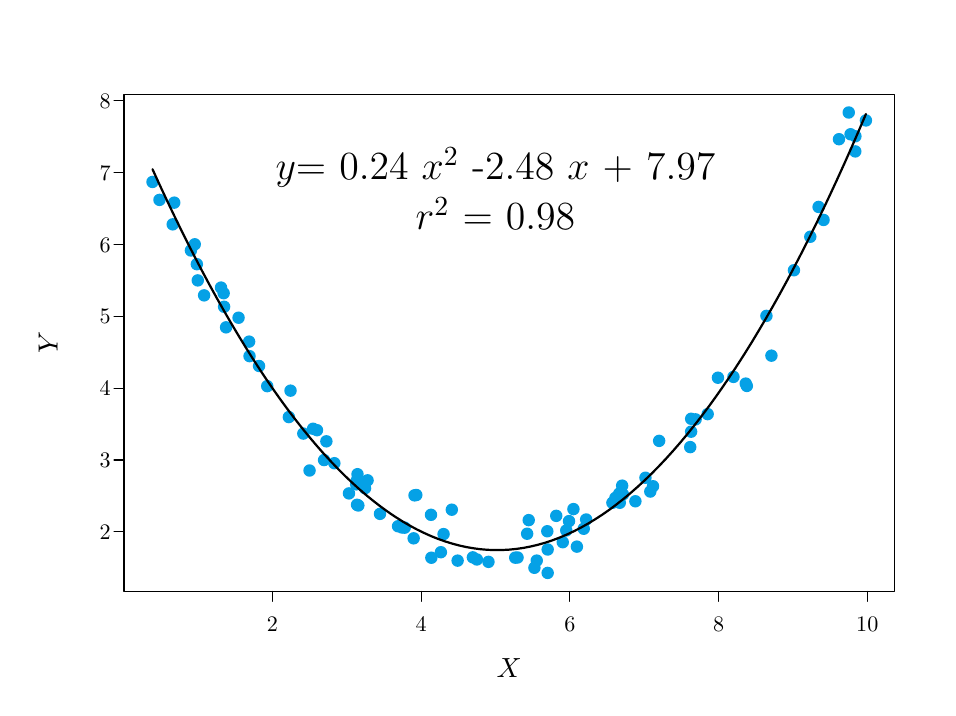
\begin{tikzpicture}[x=1pt,y=1pt]
\definecolor{fillColor}{RGB}{255,255,255}
\path[use as bounding box,fill=fillColor,fill opacity=0.00] (0,0) rectangle (325.21,238.49);
\begin{scope}
\path[clip] ( 34.80, 34.80) rectangle (313.21,214.49);
\definecolor{fillColor}{RGB}{5,161,230}

\path[fill=fillColor] ( 58.99,157.98) circle (  2.25);

\path[fill=fillColor] (139.47, 53.96) circle (  2.25);

\path[fill=fillColor] (297.34,199.97) circle (  2.25);

\path[fill=fillColor] (282.80,162.94) circle (  2.25);

\path[fill=fillColor] (119.48, 65.83) circle (  2.25);

\path[fill=fillColor] (287.59,169.01) circle (  2.25);

\path[fill=fillColor] (241.36, 96.94) circle (  2.25);

\path[fill=fillColor] (135.27, 57.88) circle (  2.25);

\path[fill=fillColor] (104.54, 93.04) circle (  2.25);

\path[fill=fillColor] (239.73, 92.50) circle (  2.25);

\path[fill=fillColor] (249.43,112.00) circle (  2.25);

\path[fill=fillColor] (195.62, 60.18) circle (  2.25);

\path[fill=fillColor] (119.18, 77.13) circle (  2.25);

\path[fill=fillColor] ( 83.60,116.24) circle (  2.25);

\path[fill=fillColor] (103.13, 93.56) circle (  2.25);

\path[fill=fillColor] (116.10, 70.20) circle (  2.25);

\path[fill=fillColor] (166.50, 45.46) circle (  2.25);

\path[fill=fillColor] (107.93, 89.02) circle (  2.25);

\path[fill=fillColor] (127.31, 62.80) circle (  2.25);

\path[fill=fillColor] (160.87, 47.09) circle (  2.25);

\path[fill=fillColor] ( 52.41,167.42) circle (  2.25);

\path[fill=fillColor] (201.81, 60.77) circle (  2.25);

\path[fill=fillColor] ( 61.13,153.03) circle (  2.25);

\path[fill=fillColor] (145.87, 46.96) circle (  2.25);

\path[fill=fillColor] (296.69,207.84) circle (  2.25);

\path[fill=fillColor] ( 52.95,175.26) circle (  2.25);

\path[fill=fillColor] (255.03,112.30) circle (  2.25);

\path[fill=fillColor] ( 69.87,144.57) circle (  2.25);

\path[fill=fillColor] ( 45.11,182.74) circle (  2.25);

\path[fill=fillColor] ( 70.81,142.54) circle (  2.25);

\path[fill=fillColor] (285.80,173.71) circle (  2.25);

\path[fill=fillColor] (239.41, 86.93) circle (  2.25);

\path[fill=fillColor] (213.96, 66.81) circle (  2.25);

\path[fill=fillColor] (122.82, 74.92) circle (  2.25);

\path[fill=fillColor] (187.90, 41.46) circle (  2.25);

\path[fill=fillColor] (118.71, 73.47) circle (  2.25);

\path[fill=fillColor] (183.95, 45.92) circle (  2.25);

\path[fill=fillColor] (194.62, 56.82) circle (  2.25);

\path[fill=fillColor] (153.26, 64.31) circle (  2.25);

\path[fill=fillColor] (119.02, 66.08) circle (  2.25);

\path[fill=fillColor] (145.74, 62.46) circle (  2.25);

\path[fill=fillColor] ( 70.98,137.64) circle (  2.25);

\path[fill=fillColor] (110.82, 81.11) circle (  2.25);

\path[fill=fillColor] (215.10, 69.84) circle (  2.25);

\path[fill=fillColor] (259.87,109.04) circle (  2.25);

\path[fill=fillColor] (191.00, 62.09) circle (  2.25);

\path[fill=fillColor] (155.36, 45.90) circle (  2.25);

\path[fill=fillColor] (214.81, 73.00) circle (  2.25);

\path[fill=fillColor] ( 63.75,141.76) circle (  2.25);

\path[fill=fillColor] (139.78, 69.49) circle (  2.25);

\path[fill=fillColor] (176.18, 46.98) circle (  2.25);

\path[fill=fillColor] (133.84, 58.33) circle (  2.25);

\path[fill=fillColor] (211.29, 66.80) circle (  2.25);

\path[fill=fillColor] (293.16,198.18) circle (  2.25);

\path[fill=fillColor] (177.01, 47.03) circle (  2.25);

\path[fill=fillColor] (181.05, 60.54) circle (  2.25);

\path[fill=fillColor] (150.28, 55.49) circle (  2.25);

\path[fill=fillColor] ( 61.47,147.17) circle (  2.25);

\path[fill=fillColor] (213.75, 70.13) circle (  2.25);

\path[fill=fillColor] ( 80.02,125.04) circle (  2.25);

\path[fill=fillColor] (193.35, 52.56) circle (  2.25);

\path[fill=fillColor] (187.90, 49.93) circle (  2.25);

\path[fill=fillColor] ( 71.69,130.20) circle (  2.25);

\path[fill=fillColor] (183.11, 43.32) circle (  2.25);

\path[fill=fillColor] ( 47.63,176.26) circle (  2.25);

\path[fill=fillColor] (200.93, 57.43) circle (  2.25);

\path[fill=fillColor] ( 94.98,107.32) circle (  2.25);

\path[fill=fillColor] (140.43, 69.62) circle (  2.25);

\path[fill=fillColor] (136.24, 57.82) circle (  2.25);

\path[fill=fillColor] ( 60.37,160.21) circle (  2.25);

\path[fill=fillColor] (225.96, 72.79) circle (  2.25);

\path[fill=fillColor] (266.95,134.35) circle (  2.25);

\path[fill=fillColor] ( 94.38, 97.78) circle (  2.25);

\path[fill=fillColor] ( 99.60, 91.82) circle (  2.25);

\path[fill=fillColor] (149.31, 48.94) circle (  2.25);

\path[fill=fillColor] ( 86.56,108.95) circle (  2.25);

\path[fill=fillColor] (107.10, 82.25) circle (  2.25);

\path[fill=fillColor] (101.86, 78.47) circle (  2.25);

\path[fill=fillColor] (224.98, 70.87) circle (  2.25);

\path[fill=fillColor] (121.91, 72.08) circle (  2.25);

\path[fill=fillColor] (212.38, 68.58) circle (  2.25);

\path[fill=fillColor] (239.75, 97.16) circle (  2.25);

\path[fill=fillColor] (228.18, 89.18) circle (  2.25);

\path[fill=fillColor] ( 80.17,119.79) circle (  2.25);

\path[fill=fillColor] (197.21, 64.53) circle (  2.25);

\path[fill=fillColor] (259.47,109.88) circle (  2.25);

\path[fill=fillColor] (245.71, 98.85) circle (  2.25);

\path[fill=fillColor] (162.32, 46.32) circle (  2.25);

\path[fill=fillColor] (302.90,204.96) circle (  2.25);

\path[fill=fillColor] (299.05,193.77) circle (  2.25);

\path[fill=fillColor] (276.89,150.83) circle (  2.25);

\path[fill=fillColor] (118.93, 74.87) circle (  2.25);

\path[fill=fillColor] (299.10,199.25) circle (  2.25);

\path[fill=fillColor] (198.46, 50.96) circle (  2.25);

\path[fill=fillColor] (180.48, 55.62) circle (  2.25);

\path[fill=fillColor] ( 76.20,133.68) circle (  2.25);

\path[fill=fillColor] (223.23, 75.85) circle (  2.25);

\path[fill=fillColor] (268.75,119.97) circle (  2.25);

\path[fill=fillColor] (219.60, 67.35) circle (  2.25);

\path[fill=fillColor] (187.77, 56.52) circle (  2.25);
\end{scope}
\begin{scope}
\path[clip] (  0.00,  0.00) rectangle (325.21,238.49);
\definecolor{drawColor}{RGB}{0,0,0}

\path[draw=drawColor,line width= 0.4pt,line join=round,line cap=round] ( 88.41, 34.80) -- (303.39, 34.80);

\path[draw=drawColor,line width= 0.4pt,line join=round,line cap=round] ( 88.41, 34.80) -- ( 88.41, 31.21);

\path[draw=drawColor,line width= 0.4pt,line join=round,line cap=round] (142.16, 34.80) -- (142.16, 31.21);

\path[draw=drawColor,line width= 0.4pt,line join=round,line cap=round] (195.90, 34.80) -- (195.90, 31.21);

\path[draw=drawColor,line width= 0.4pt,line join=round,line cap=round] (249.65, 34.80) -- (249.65, 31.21);

\path[draw=drawColor,line width= 0.4pt,line join=round,line cap=round] (303.39, 34.80) -- (303.39, 31.21);

\node[text=drawColor,anchor=base,inner sep=0pt, outer sep=0pt, scale=  0.80] at ( 88.41, 20.40) {2};

\node[text=drawColor,anchor=base,inner sep=0pt, outer sep=0pt, scale=  0.80] at (142.16, 20.40) {4};

\node[text=drawColor,anchor=base,inner sep=0pt, outer sep=0pt, scale=  0.80] at (195.90, 20.40) {6};

\node[text=drawColor,anchor=base,inner sep=0pt, outer sep=0pt, scale=  0.80] at (249.65, 20.40) {8};

\node[text=drawColor,anchor=base,inner sep=0pt, outer sep=0pt, scale=  0.80] at (303.39, 20.40) {10};

\path[draw=drawColor,line width= 0.4pt,line join=round,line cap=round] ( 34.80, 56.32) -- ( 34.80,212.09);

\path[draw=drawColor,line width= 0.4pt,line join=round,line cap=round] ( 34.80, 56.32) -- ( 31.21, 56.32);

\path[draw=drawColor,line width= 0.4pt,line join=round,line cap=round] ( 34.80, 82.28) -- ( 31.21, 82.28);

\path[draw=drawColor,line width= 0.4pt,line join=round,line cap=round] ( 34.80,108.25) -- ( 31.21,108.25);

\path[draw=drawColor,line width= 0.4pt,line join=round,line cap=round] ( 34.80,134.21) -- ( 31.21,134.21);

\path[draw=drawColor,line width= 0.4pt,line join=round,line cap=round] ( 34.80,160.17) -- ( 31.21,160.17);

\path[draw=drawColor,line width= 0.4pt,line join=round,line cap=round] ( 34.80,186.13) -- ( 31.21,186.13);

\path[draw=drawColor,line width= 0.4pt,line join=round,line cap=round] ( 34.80,212.09) -- ( 31.21,212.09);

\node[text=drawColor,anchor=base east,inner sep=0pt, outer sep=0pt, scale=  0.80] at ( 30.00, 53.57) {2};

\node[text=drawColor,anchor=base east,inner sep=0pt, outer sep=0pt, scale=  0.80] at ( 30.00, 79.53) {3};

\node[text=drawColor,anchor=base east,inner sep=0pt, outer sep=0pt, scale=  0.80] at ( 30.00,105.49) {4};

\node[text=drawColor,anchor=base east,inner sep=0pt, outer sep=0pt, scale=  0.80] at ( 30.00,131.45) {5};

\node[text=drawColor,anchor=base east,inner sep=0pt, outer sep=0pt, scale=  0.80] at ( 30.00,157.41) {6};

\node[text=drawColor,anchor=base east,inner sep=0pt, outer sep=0pt, scale=  0.80] at ( 30.00,183.37) {7};

\node[text=drawColor,anchor=base east,inner sep=0pt, outer sep=0pt, scale=  0.80] at ( 30.00,209.33) {8};

\path[draw=drawColor,line width= 0.4pt,line join=round,line cap=round] ( 34.80, 34.80) --
	(313.21, 34.80) --
	(313.21,214.49) --
	( 34.80,214.49) --
	( 34.80, 34.80);
\end{scope}
\begin{scope}
\path[clip] (  0.00,  0.00) rectangle (325.21,238.49);
\definecolor{drawColor}{RGB}{0,0,0}

\node[text=drawColor,anchor=base,inner sep=0pt, outer sep=0pt, scale=  1.00] at (174.01,  3.60) {$X$};

\node[text=drawColor,rotate= 90.00,anchor=base,inner sep=0pt, outer sep=0pt, scale=  1.00] at ( 10.80,124.65) {$Y$};
\end{scope}
\begin{scope}
\path[clip] ( 34.80, 34.80) rectangle (313.21,214.49);
\definecolor{drawColor}{RGB}{0,0,0}

\path[draw=drawColor,line width= 0.8pt,line join=round,line cap=round] ( 45.11,187.33) --
	( 47.69,181.69) --
	( 50.27,176.17) --
	( 52.85,170.77) --
	( 55.42,165.48) --
	( 58.00,160.31) --
	( 60.58,155.27) --
	( 63.16,150.33) --
	( 65.73,145.52) --
	( 68.31,140.83) --
	( 70.89,136.25) --
	( 73.47,131.79) --
	( 76.05,127.45) --
	( 78.62,123.23) --
	( 81.20,119.12) --
	( 83.78,115.13) --
	( 86.36,111.26) --
	( 88.94,107.51) --
	( 91.51,103.88) --
	( 94.09,100.36) --
	( 96.67, 96.97) --
	( 99.25, 93.69) --
	(101.83, 90.52) --
	(104.40, 87.48) --
	(106.98, 84.55) --
	(109.56, 81.75) --
	(112.14, 79.06) --
	(114.72, 76.48) --
	(117.29, 74.03) --
	(119.87, 71.69) --
	(122.45, 69.48) --
	(125.03, 67.38) --
	(127.61, 65.39) --
	(130.18, 63.53) --
	(132.76, 61.78) --
	(135.34, 60.15) --
	(137.92, 58.64) --
	(140.49, 57.25) --
	(143.07, 55.98) --
	(145.65, 54.82) --
	(148.23, 53.78) --
	(150.81, 52.86) --
	(153.38, 52.06) --
	(155.96, 51.37) --
	(158.54, 50.80) --
	(161.12, 50.36) --
	(163.70, 50.02) --
	(166.27, 49.81) --
	(168.85, 49.72) --
	(171.43, 49.74) --
	(174.01, 49.88) --
	(176.59, 50.14) --
	(179.16, 50.51) --
	(181.74, 51.01) --
	(184.32, 51.62) --
	(186.90, 52.35) --
	(189.47, 53.20) --
	(192.05, 54.17) --
	(194.63, 55.25) --
	(197.21, 56.45) --
	(199.79, 57.77) --
	(202.36, 59.21) --
	(204.94, 60.77) --
	(207.52, 62.44) --
	(210.10, 64.23) --
	(212.68, 66.14) --
	(215.25, 68.17) --
	(217.83, 70.32) --
	(220.41, 72.58) --
	(222.99, 74.96) --
	(225.57, 77.46) --
	(228.14, 80.08) --
	(230.72, 82.81) --
	(233.30, 85.67) --
	(235.88, 88.64) --
	(238.46, 91.73) --
	(241.03, 94.94) --
	(243.61, 98.26) --
	(246.19,101.70) --
	(248.77,105.27) --
	(251.34,108.94) --
	(253.92,112.74) --
	(256.50,116.66) --
	(259.08,120.69) --
	(261.66,124.84) --
	(264.23,129.11) --
	(266.81,133.50) --
	(269.39,138.00) --
	(271.97,142.62) --
	(274.55,147.36) --
	(277.12,152.22) --
	(279.70,157.20) --
	(282.28,162.29) --
	(284.86,167.51) --
	(287.44,172.84) --
	(290.01,178.28) --
	(292.59,183.85) --
	(295.17,189.53) --
	(297.75,195.34) --
	(300.33,201.26) --
	(302.90,207.29);

\node[text=drawColor,anchor=base,inner sep=0pt, outer sep=0pt, scale=  1.00] at (169.03,183.63) {\Large $y$= 0.24 $x^2$ -2.48 $x$ + 7.97};

\node[text=drawColor,anchor=base,inner sep=0pt, outer sep=0pt, scale=  1.00] at (169.03,165.45) {\Large $r^2$ = 0.98};
\end{scope}
\end{tikzpicture}
